\documentclass[11pt]{article}

% ---------------------------------------------------------------------------
%  Plain-language guide to the KT-D1V5 Sod shock-tube solver.
%  The full technical version is d1v5_solver_mathematics.tex.
%  Build:  tectonic d1v5_solver_simple_guide.tex
% ---------------------------------------------------------------------------

\usepackage[letterpaper,margin=1in]{geometry}
\usepackage[T1]{fontenc}
\usepackage{lmodern}
\usepackage{microtype}
\usepackage{amsmath,amssymb}
\usepackage{graphicx}
\usepackage{booktabs}
\usepackage{xcolor}
\usepackage{caption}
\usepackage{enumitem}
\usepackage{tikz}
\usetikzlibrary{arrows.meta,decorations.pathreplacing}
\usepackage[numbers,sort&compress]{natbib}
\usepackage[colorlinks=true,linkcolor=blue!50!black,citecolor=blue!50!black,urlcolor=blue!50!black]{hyperref}
\usepackage{cleveref}
\usepackage{tcolorbox}
\usepackage[section]{placeins}

\captionsetup{font=small,labelfont=bf}
\setlist{itemsep=3pt,topsep=4pt}
\graphicspath{{figures/}}
\setlength{\parskip}{4pt}

\newcommand{\feq}{f^{\mathrm{eq}}}
\newtcolorbox{idea}{colback=blue!4,colframe=blue!45!black,boxrule=0.6pt,arc=2pt,left=6pt,right=6pt,top=4pt,bottom=4pt}

\title{\textbf{How the KT-D1V5 Shock-Tube Solver Works}\\[4pt]
\large A plain-language guide to the math and physics}
\author{Nathan Kidwell}
\date{September 2026}

\begin{document}
\maketitle

\begin{idea}
\textbf{The short version.}
The solver does not compute density, velocity and pressure directly.  It tracks
five groups of imaginary gas particles, each moving at a fixed speed.  In every
time step the particles
\begin{enumerate}[leftmargin=18pt]
  \item \textbf{move} left or right through small cells of the tube, and
  \item \textbf{collide}, which nudges each group toward a ``balanced'' amount
        (the equilibrium).
\end{enumerate}
Adding the groups up in the right ways gives the density, velocity, temperature
and pressure of the gas.  This guide explains each piece, then shows how well the
result matches the exact answer for the Sod shock tube.
\end{idea}

\tableofcontents

% ===========================================================================
\section{The problem: the Sod shock tube}
% ===========================================================================

Picture a long tube, 20 units long, with a thin wall in the middle ($x = 10$).
The left side holds dense, high-pressure gas and the right side holds thin,
low-pressure gas:
\[
\text{left: } \rho = 1,\ u = 0,\ p = 1 \qquad\qquad
\text{right: } \rho = 0.125,\ u = 0,\ p = 0.1 .
\]
Here $\rho$ is density, $u$ is flow velocity and $p$ is pressure.  At time zero the
wall disappears.  By the final time $t = 0.15$ three waves have formed
(\cref{fig:sod}):
\begin{itemize}
  \item a \textbf{rarefaction} (expansion fan) moving left, where the gas smoothly
        thins out;
  \item a \textbf{contact}, the boundary between the ``old left gas'' and the
        ``old right gas''.  Density and temperature jump here, but pressure and
        velocity do not;
  \item a \textbf{shock} moving right, where all four quantities jump.
\end{itemize}

This problem is a standard test because its exact answer is known~\citep{Sod1978,Toro2009}.
The exact values used for comparison are listed in \cref{tab:sod}.  The main ones
are a middle-region pressure $p^* = 0.3031$, a flow speed $u^* = 0.9275$, and a
shock speed of $1.752$.

\begin{figure}[!htbp]
\centering
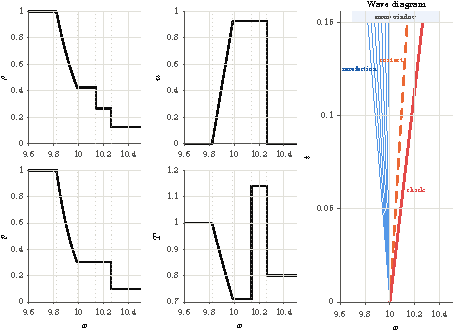
\includegraphics[width=\textwidth]{fig_exact_sod.pdf}
\caption{The exact answer at $t = 0.15$.  Left: density, velocity, pressure and
temperature along the tube (dotted lines mark the waves).  Right: the paths of the
waves in time.  The shaded strip is the region used to measure errors.}
\label{fig:sod}
\end{figure}

\begin{table}[!htbp]
\centering
\caption{Exact Sod values at $t = 0.15$ (gas with $\gamma = 1.4$).}
\label{tab:sod}
\small
\begin{tabular}{@{}lll@{}}
\toprule
Quantity & Value & Meaning \\
\midrule
$p^*$, $u^*$ & $0.3031$, $0.9275$ & middle-region pressure and speed\\
$\rho$ left / right of contact & $0.4263$ / $0.2656$ & density jumps at the contact\\
$T$ left / right of contact & $0.711$ / $1.141$ & temperature jumps at the contact\\
Shock speed & $1.752$ (Mach 1.66) & shock is $0.263$ right of the wall\\
Contact position & $0.139$ right of the wall & moves with the gas\\
Rarefaction & $0.177$ to $0.011$ left of wall & smooth expansion\\
\bottomrule
\end{tabular}
\end{table}

% ===========================================================================
\section{The physics idea: particles instead of fluid}
% ===========================================================================

\subsection{The Boltzmann--BGK equation}
Gas is made of molecules moving in all directions.  Kinetic theory describes the gas
by a \emph{distribution} $f$: how many molecules are at each place moving at each
speed.  The simplest useful model of how $f$ changes is the BGK
equation~\citep{BGK1954}:
\begin{equation}
  \underbrace{\frac{\partial f}{\partial t}}_{\text{change in time}}
  + \underbrace{c\,\frac{\partial f}{\partial x}}_{\text{particles moving}}
  = \underbrace{\frac{\feq - f}{\tau}}_{\text{collisions}} .
  \label{eq:bgk}
\end{equation}
The left side says that particles with speed $c$ simply drift along the tube.  The
right side says that collisions pull $f$ toward a balanced shape $\feq$ (the
\emph{equilibrium}).  The \textbf{relaxation time} $\tau$ sets how fast that happens.

\begin{idea}
\textbf{What $\tau$ means.}  $\tau$ is roughly the time between collisions.  A small
$\tau$ means the gas re-balances almost instantly and behaves like an ideal
(frictionless) fluid.  A larger $\tau$ adds a little ``stickiness'' (viscosity) that
smooths sharp jumps.  This solver uses $\tau = 5\times10^{-6}$, which is very small.
\end{idea}

When $\tau$ is small, averaging~\eqref{eq:bgk} over all particles gives back the
ordinary \textbf{Euler equations} of gas dynamics (conservation of mass, momentum
and energy)~\citep{ChapmanCowling1970}.  That is why a particle model can solve a
fluid problem.

\subsection{Only five particle speeds: the D1V5 model}
A real gas has every speed.  The solver keeps only \textbf{five}
(\cref{fig:velset}), following Kataoka and Tsutahara~\citep{KataokaTsutahara2004Euler}:
\[
c \in \{-3,\ -1,\ 0,\ +1,\ +3\}.
\]
``D1V5'' means one dimension, five velocities.  The group with speed $0$ does not
move, but it carries an extra energy ``backpack'' ($\eta_0 = 1.75$).  That backpack
stands in for the energy a real molecule stores in spinning and in sideways motion,
which is what lets the model represent air ($\gamma = 1.4$).

\begin{figure}[!htbp]
\centering
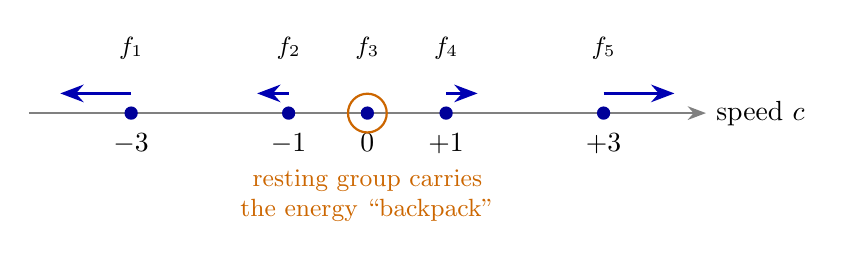
\begin{tikzpicture}[>=Stealth]
  \draw[->,thick,gray] (-4.3,0) -- (4.3,0) node[right,black] {speed $c$};
  \foreach \x/\lab/\idx in {-3/{-3}/1,-1/{-1}/2,0/{0}/3,1/{+1}/4,3/{+3}/5}{
    \fill[blue!60!black] (\x,0) circle (2.4pt);
    \node[below=4pt] at (\x,0) {$\lab$};
    \node[above=16pt,font=\small] at (\x,0) {$f_{\idx}$};
  }
  \draw[->,very thick,blue!70!black] (-3,0.25) -- (-3.9,0.25);
  \draw[->,very thick,blue!70!black] (-1,0.25) -- (-1.4,0.25);
  \draw[->,very thick,blue!70!black] (1,0.25) -- (1.4,0.25);
  \draw[->,very thick,blue!70!black] (3,0.25) -- (3.9,0.25);
  \draw[orange!80!black,thick] (0,0) circle (7pt);
  \node[orange!80!black,font=\small,align=center] at (0,-1.05) {resting group carries\\ the energy ``backpack''};
\end{tikzpicture}
\caption{The five particle groups.  Arrows show their direction and relative speed.}
\label{fig:velset}
\end{figure}

\subsection{Getting density, velocity, temperature and pressure back}
Each cell stores five numbers, $f_1,\dots,f_5$.  The gas properties come from
weighted sums of them:
\begin{align*}
  \rho &= f_1 + f_2 + f_3 + f_4 + f_5 &&\text{(total amount $=$ density)}\\
  \rho u &= \textstyle\sum_i c_i f_i &&\text{(speed-weighted sum $=$ momentum)}\\
  \rho\,(5T + u^2) &= \textstyle\sum_i (c_i^2 + \eta_i^2) f_i &&\text{(energy)}\\
  p &= \rho T &&\text{(ideal-gas law)}
\end{align*}
Temperature is found last: take the total energy and subtract the part that is just
bulk motion ($u^2$).  Because it is a difference of two large numbers, $T$ is the
most sensitive result.  A small error in one group (especially a fast group) shows
up in $T$ more strongly than in $\rho$ or $p$.  This is why temperature shows
overshoots first (\cref{sec:limiters_results}).

\subsection{The equilibrium}
The balanced state $\feq$ is not guessed.  Its five values are chosen so that they
give back exactly the right density, momentum and energy, and also the right
\emph{flow} of momentum and energy that the Euler equations need.  Those are five
conditions for five unknowns, so there is exactly one answer.  It is the formula in
the solver's equilibrium function.  I checked it numerically on 2000 random gas
states; it reproduces all five quantities to about $10^{-15}$.

Two facts worth knowing:
\begin{itemize}
  \item Some equilibrium values are \textbf{negative} (the slow groups, for the
        temperatures in this problem).  That is allowed: the groups are
        bookkeeping quantities, not real particle counts.  It is also why the
        solver checks that $\rho$ and $T$ stay positive rather than checking each
        $f_i$.
  \item Mass, momentum and energy are \textbf{never created or destroyed} by
        collisions, because the equilibrium is built from the same totals as $f$.
\end{itemize}

% ===========================================================================
\section{How the computer solves it}
% ===========================================================================

The solver repeats the same step many times until $t = 0.15$.  Each step has three
ingredients.

\subsection{Ingredient 1: cells and fluxes (finite volumes)}
The tube is cut into $N_x$ equal cells of width $\Delta x = 20/N_x$.  For example,
$N_x = 50{,}000$ gives $\Delta x = 0.0004$.  Each cell stores the average $f_i$
inside it.  A cell's value changes only because of what flows in and out through
its two walls, plus collisions:
\[
  \text{change in cell} = -\frac{\text{flux out right wall} - \text{flux in left wall}}{\Delta x} + \frac{\feq - f}{\tau}.
\]
Whatever leaves one cell enters its neighbour, so nothing is lost.  The results
confirm this: total mass and energy stay constant to about $10^{-12}$.

\subsection{Ingredient 2: upwinding, and MUSCL for sharper answers}
To find the flux through a wall, you need the value of $f_i$ right at that wall.
Because each group moves in one direction only, the rule is simple
(\cref{fig:muscl}):
\begin{itemize}
  \item right-moving groups ($c = +1, +3$) take the value from the cell on the
        \emph{left} of the wall;
  \item left-moving groups ($c = -1, -3$) take it from the cell on the \emph{right};
  \item the resting group ($c = 0$) never crosses a wall.
\end{itemize}
This is called \textbf{upwinding}: you look ``upstream'' for the information.

Using the plain cell average at the wall (``first-order'') is stable but smears
every jump over many cells.  \textbf{MUSCL}~\citep{vanLeer1979} does better.  It
draws a sloped line through each cell and reads the wall value off that line:
\[
  \text{value at right wall of cell } j = f_j + \tfrac12\,\sigma_j ,
\]
where $\sigma_j$ is the slope (the change across one cell).

\begin{figure}[!htbp]
\centering
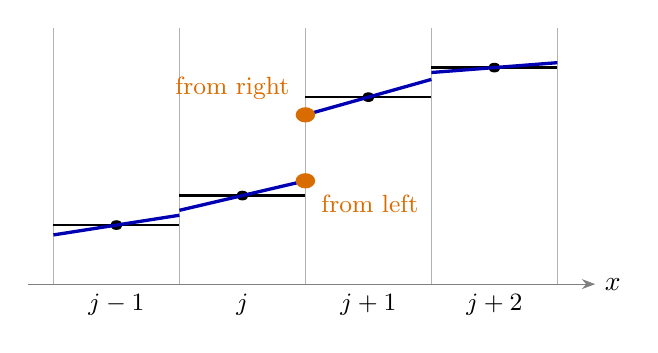
\begin{tikzpicture}[>=Stealth,xscale=1.6,yscale=1.25]
  \foreach \i in {0,...,4}{ \draw[gray!60] (\i,0) -- (\i,2.6); }
  \draw[->,gray] (-0.2,0) -- (4.3,0) node[right,black] {$x$};
  \node[below,font=\small] at (0.5,0) {$j-1$};
  \node[below,font=\small] at (1.5,0) {$j$};
  \node[below,font=\small] at (2.5,0) {$j+1$};
  \node[below,font=\small] at (3.5,0) {$j+2$};
  \foreach \x/\y in {0.5/0.6,1.5/0.9,2.5/1.9,3.5/2.2}{
    \draw[thick,black] (\x-0.5,\y) -- (\x+0.5,\y);
    \fill (\x,\y) circle (1.4pt);
  }
  \draw[very thick,blue!70!black] (1,0.75) -- (2,1.05);
  \draw[very thick,blue!70!black] (2,1.72) -- (3,2.08);
  \draw[very thick,blue!70!black] (0,0.5) -- (1,0.7);
  \draw[very thick,blue!70!black] (3,2.15) -- (4,2.25);
  \fill[orange!85!black] (2,1.05) circle (2.2pt);
  \node[orange!85!black,font=\small,anchor=north west] at (2.05,1.0) {from left};
  \fill[orange!85!black] (2,1.72) circle (2.2pt);
  \node[orange!85!black,font=\small,anchor=south east] at (1.95,1.78) {from right};
\end{tikzpicture}
\caption{MUSCL.  Black: cell averages.  Blue: sloped lines inside each cell.
Orange: the two possible values at the wall between cells $j$ and $j{+}1$.
Right-moving groups use the ``from left'' value; left-moving groups use the ``from
right'' value.}
\label{fig:muscl}
\end{figure}

\subsection{Ingredient 3: the slope limiter (generalized minmod)}
A slope that is too steep near a jump creates fake wiggles (overshoots).  A
\textbf{limiter} decides how steep the slope may be.  Let $d_L$ be the change from
the left neighbour and $d_R$ the change to the right neighbour.  The solver uses
the \textbf{generalized minmod} limiter~\citep{KurganovTadmor2000}:
\[
  \sigma = \operatorname{minmod}\!\Big(\theta\, d_L,\ \tfrac12(d_L + d_R),\ \theta\, d_R\Big),
  \qquad \theta = 1.2 .
\]
``minmod'' means: if all three candidates have the same sign, pick the one closest
to zero; if the signs disagree (a peak or a dip), use a slope of zero.  So:
\begin{itemize}
  \item at a peak or dip the slope is switched off, which prevents new wiggles;
  \item in smooth regions the slope is the smallest of three reasonable estimates;
  \item $\theta$ is a dial.  $\theta = 1$ is plain \emph{minmod} (very safe, but
        smears jumps).  $\theta = 2$ is \emph{MC} (sharp, but overshoots).
        $\theta = 1.2$ sits in between.
\end{itemize}
Theory~\citep{Sweby1984,Harten1983} shows this family never creates new wiggles in
a single group's motion as long as $1 \le \theta \le 2$, which is why $\theta$ is
kept in that range (\cref{fig:sweby}).

\begin{figure}[!htbp]
\centering
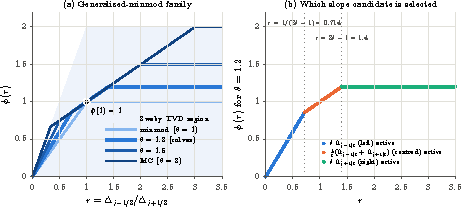
\includegraphics[width=\textwidth]{fig_sweby_diagram.pdf}
\caption{(a) How steep the slope is allowed to be for different $\theta$.  The
horizontal axis measures how smooth the data are ($r = 1$ means perfectly smooth).
All curves stay inside the shaded ``no-new-wiggles'' region.  (b) Which of the
three candidates $\theta = 1.2$ picks.}
\label{fig:sweby}
\end{figure}

\subsection{Moving forward in time: SSP-RK3}
Instead of one big jump per step, the solver takes three smaller ``looks'' and
blends them (the SSP Runge--Kutta method of Shu and Osher~\citep{ShuOsher1988}).
Writing $L(f)$ for ``movement plus collisions'':
\begin{align*}
  f^{(1)} &= f^n + \Delta t\,L(f^n)\\
  f^{(2)} &= \tfrac34 f^n + \tfrac14\big[f^{(1)} + \Delta t\,L(f^{(1)})\big]\\
  f^{n+1} &= \tfrac13 f^n + \tfrac23\big[f^{(2)} + \Delta t\,L(f^{(2)})\big]
\end{align*}
Each line is an average of simple forward steps.  That keeps the good ``no new
wiggles'' behaviour of the limiter while being much more accurate than a single
forward step.

\paragraph{How big is each time step?}  Two limits are checked and the smaller one
is used:
\[
  \Delta t = \min\Big(\underbrace{\text{CFL}\cdot\frac{\Delta x}{3}}_{\text{movement limit}},\ \ \underbrace{\tau/4}_{\text{collision limit}}\Big).
\]
The movement limit keeps the fastest group from jumping too far in one step.  The
collision limit keeps the relaxation accurate.  With $\tau = 5\times10^{-6}$, the
collision limit gives $\Delta t = 1.25\times10^{-6}$, and that is smaller than the
movement limit on \emph{every} grid used here, even with CFL $= 0.025$.  So every run
used the same time step and the same $120{,}000$ steps.  In practice the CFL setting
never controlled the step.

\paragraph{Safety checks.}  After each stage the solver checks that density and
temperature are still positive.  If not, it halves the time step and, if needed,
switches to a safer limiter.  In every run reported here this \emph{never
happened}: zero retries, zero fallbacks.

% ===========================================================================
\section{What $\tau$ does to the answer}
% ===========================================================================

The exact Sod answer assumes a perfectly frictionless gas ($\tau = 0$).  The solver
uses a small but nonzero $\tau$, so even a perfect computer would give slightly
smoothed jumps.  Working through the math for this five-speed model shows the
following.
\begin{itemize}
  \item The \textbf{shock} is smoothed only over about $7\tau \approx 0.00004$,
        which is much thinner than one cell.  The shock's width in the results
        comes from the grid, not from $\tau$.
  \item The \textbf{contact} keeps spreading with time, like heat diffusing.  By
        $t = 0.15$ its natural width is about $0.0012$--$0.0015$, roughly three
        cells on the finest grid.
  \item The spreading rate at the contact depends on how fast the gas is moving
        there.  At the Sod contact ($u \approx 0.93$) it is about 8 times slower
        than for gas at rest.  If the gas moved faster than the slow particle
        speed ($u > 1$), the model would break down.  So this velocity set is only
        suitable for flows slower than that.
\end{itemize}
The practical meaning: refining the grid can only help until the cells are smaller
than this natural contact width.  For $\tau = 5\times10^{-6}$ that happens around
$N_x \approx 200{,}000$ cells.  For the older $\tau = 5\times10^{-5}$ it happens
around $50{,}000$ cells, which explains why the earlier study stopped improving
there.

% ===========================================================================
\section{How accuracy is measured}
% ===========================================================================

At each cell the numerical value is compared with the exact value.
\begin{itemize}
  \item \textbf{$L_1$ error}: the average size of the miss over all cells.
  \item \textbf{$L_2$ error}: the root-mean-square miss.  It punishes large local
        misses more than $L_1$ does.
  \item \textbf{Temperature peak excess}: highest computed temperature minus the
        highest exact temperature.  A positive value means an overshoot.
  \item \textbf{Order of convergence} $p$: how fast the error shrinks when the cells
        get smaller.  If halving $\Delta x$ cuts the error in half, $p = 1$; if it
        cuts it by a quarter, $p = 2$.  It is computed as
        \[
          p = \frac{\log(E_{\text{coarse}}/E_{\text{fine}})}{\log(\Delta x_{\text{coarse}}/\Delta x_{\text{fine}})}.
        \]
\end{itemize}

\begin{idea}
\textbf{What order to expect.}  The method is ``second order'' only where the
solution is smooth.  Sod has jumps, and every method smears a jump over a few
cells, so the error there cannot shrink as fast~\citep{LeVeque2002}.  For this kind
of method the expected orders are about:
\begin{itemize}[leftmargin=14pt]
  \item $L_1$: between $0.67$ (from the contact) and $1$ (from the shock);
  \item $L_2$: between $0.33$ (contact) and $0.5$ (shock).
\end{itemize}
So an $L_2$ order around $0.4$--$0.5$ is \emph{normal and correct} here.  It does
not mean something is wrong.
\end{idea}

% ===========================================================================
\section{Results}
% ===========================================================================

Settings for every run: $\tau = 5\times10^{-6}$, CFL $= 0.025$, $\theta = 1.2$, final
time $0.15$, tube length $20$.

\subsection{The solution looks right}
\Cref{fig:finest} shows the finest grid (50,000 cells) against the exact answer.
All four quantities match closely with no wiggles.  The errors are concentrated in
a few cells at the contact and the shock, as expected.  \Cref{fig:zoom} zooms in
on each wave: every grid refinement makes the jumps sharper.

\begin{figure}[!htbp]
\centering
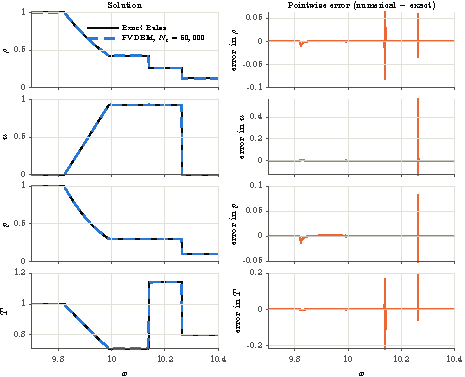
\includegraphics[width=\textwidth]{fig_solution_finest.pdf}
\caption{Finest grid (dashed blue) versus the exact answer (black), with the
point-by-point error on the right.}
\label{fig:finest}
\end{figure}

\begin{figure}[!htbp]
\centering
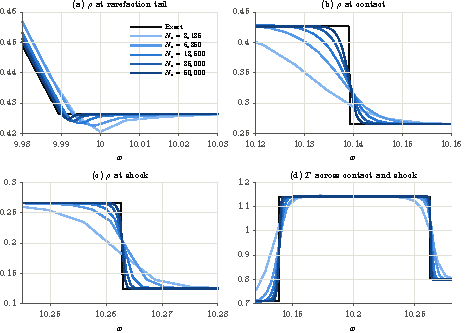
\includegraphics[width=\textwidth]{fig_grid_zoom.pdf}
\caption{Close-ups at each wave.  Darker blue means more cells.  The shock stays
about 3 cells wide.  The contact is wider, and the small temperature overshoot on
the coarsest grids disappears by 12,500 cells.}
\label{fig:zoom}
\end{figure}

\subsection{Grid convergence}

\begin{table}[!htbp]
\centering
\caption{Whole-tube $L_2$ errors and temperature peak excess.}
\label{tab:conv}
\small
\begin{tabular}{@{}rccccc@{}}
\toprule
Cells $N_x$ & $\rho$ & $u$ & $p$ & $T$ & $T$ peak excess \\
\midrule
3,125  & 0.00316 & 0.00779 & 0.00308 & 0.00592 & $+0.0039$ \\
6,250  & 0.00181 & 0.00806 & 0.00164 & 0.00465 & $+0.0016$ \\
12,500 & 0.00139 & 0.00613 & 0.00114 & 0.00354 & $\approx 0$ \\
25,000 & 0.00100 & 0.00271 & 0.00072 & 0.00244 & $\approx 0$ \\
50,000 & 0.00078 & 0.00275 & 0.00051 & 0.00202 & $\approx 0$ \\
\midrule
Order ($L_2$) & 0.49 & 0.46 & 0.63 & 0.40 & \\
Order ($L_1$) & 0.83 & 0.89 & 0.88 & 0.81 & \\
\bottomrule
\end{tabular}
\end{table}

\Cref{tab:conv} and \cref{fig:conv} give the main result.
\begin{itemize}
  \item Every error gets smaller as the grid is refined.
  \item The orders ($L_2 \approx 0.4$--$0.6$, $L_1 \approx 0.8$--$0.9$) are exactly
        in the expected range for a problem with a shock and a contact.
  \item All runs were clean: no retries, no fallbacks, and mass and energy were
        conserved to about $10^{-12}$.
  \item The \textbf{contact} is the slowest part to improve.  It limits the density
        and temperature errors.  The shock stays about 3 cells wide at every
        resolution, which is typical.
\end{itemize}

\begin{figure}[!htbp]
\centering
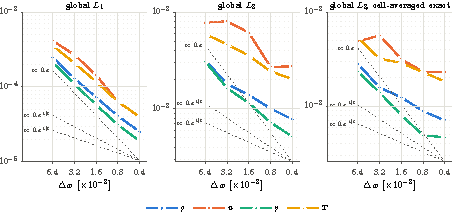
\includegraphics[width=\textwidth]{fig_convergence.pdf}
\caption{Errors versus cell size (smaller cells to the right).  Dotted lines show
reference slopes.  Lines running parallel to the $\Delta x^{1/3}$ to $\Delta x^{1/2}$
guides are the expected behaviour.}
\label{fig:conv}
\end{figure}

\subsection{Why the velocity error stopped improving from 25k to 50k cells}
Nearly all of the velocity error sits in the few cells right at the shock, where
the velocity drops from $0.93$ to $0$.  How big that error is depends on
\emph{where the exact shock happens to fall inside a cell}: near a cell's edge or
near its middle.  That position is different on every grid.  On the 25k grid the
shock sits near the middle of a cell (smaller error); on the 50k grid it sits near
an edge (larger error).  Comparing grids where the shock sits in the same spot, the
velocity error shrinks at order $0.50$--$0.51$, exactly as expected
(\cref{fig:phase}).  So the stall is a quirk of how the error is measured, not a
problem with $\tau$ or the time step.  The $L_1$ velocity error, which is less
sensitive to this, improves steadily.

\begin{figure}[!htbp]
\centering
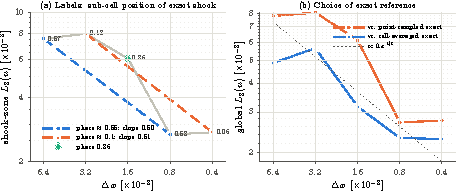
\includegraphics[width=\textwidth]{fig_shock_phase.pdf}
\caption{(a) Velocity error near the shock.  The labels give where the exact shock
falls inside its cell (0 = edge, 0.5 = middle).  Grids with matching positions
(same colour) improve at the expected rate.  (b) The whole-tube velocity error.}
\label{fig:phase}
\end{figure}

\subsection{Effect of the smaller $\tau$}
\Cref{tab:tau} compares this study with the earlier one at a 10 times larger $\tau$.
With the old $\tau$ the error levelled off near $1.13\times10^{-3}$ from 40,000 cells
on.  With the new $\tau$ it keeps dropping, reaching $0.78\times10^{-3}$ at 50,000
cells.  This matches the prediction above: the old $\tau$ made the contact
naturally wider, so the grid could no longer help.  (The earlier runs also used a
larger time step, so this comparison changes two things at once.)

\begin{table}[!htbp]
\centering
\caption{Density $L_2$ error at the old and new relaxation times.}
\label{tab:tau}
\small
\begin{tabular}{@{}rccc@{}}
\toprule
Cells & old $\tau = 5\times10^{-5}$ & new $\tau = 5\times10^{-6}$ & new / old \\
\midrule
3,125  & 0.00324 & 0.00316 & 0.97 \\
6,250  & 0.00196 & 0.00181 & 0.92 \\
12,500 & 0.00159 & 0.00139 & 0.87 \\
25,000 & 0.00126 & 0.00100 & 0.80 \\
40,000 & 0.00113 & ---     & ---  \\
50,000 & 0.00113 & 0.00078 & 0.69 \\
\bottomrule
\end{tabular}
\end{table}

\subsection{Comparing the limiters}
\label{sec:limiters_results}
All five limiters tried during the project were rerun at 6,250 cells with identical
settings (\cref{tab:lim}, \cref{fig:lim}).

\begin{table}[!htbp]
\centering
\caption{Limiter comparison, 6,250 cells.  Lower is better in both columns.}
\label{tab:lim}
\small
\begin{tabular}{@{}lcc@{}}
\toprule
Limiter & average temperature error $L_1(T)$ & temperature overshoot \\
\midrule
Minmod                     & 0.000265 & 0.00045 \\
MC                         & 0.000168 & 0.00672 \\
Population hybrid          & 0.000216 & 0.00259 \\
Macroscopic hybrid         & 0.000266 & 0.00062 \\
\textbf{Generalized minmod, $\theta = 1.2$} & \textbf{0.000208} & \textbf{0.00155} \\
\bottomrule
\end{tabular}
\end{table}

\begin{itemize}
  \item \textbf{MC} has the smallest average error but by far the largest
        temperature overshoot.
  \item \textbf{Minmod} has almost no overshoot but the largest average error.
  \item \textbf{Generalized minmod ($\theta = 1.2$)} is in between.  Compared with
        minmod, it lowers every average error by 20--23\%.  Compared with MC, it
        cuts the overshoot by 77\%.
\end{itemize}

\begin{figure}[!htbp]
\centering
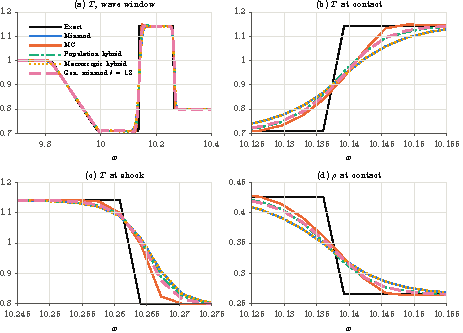
\includegraphics[width=\textwidth]{fig_limiters.pdf}
\caption{Temperature and density near the contact and shock for each limiter.
MC (orange) is sharpest but overshoots just behind the contact.}
\label{fig:lim}
\end{figure}

\subsection{Choosing $\theta$}
Running every $\theta$ from 1.0 to 2.0 (\cref{fig:theta}) shows a clean tradeoff:
as $\theta$ increases, the average error always goes down and the overshoot always
goes up.  No single $\theta$ wins on both.  $\theta = 1.2$ gets about 59\% of the
possible error reduction while paying only about 18\% of the possible overshoot.
It is a sensible middle choice, not a ``perfect'' value.  On finer grids the
overshoot at $\theta = 1.2$ disappears anyway (\cref{tab:conv}).

\begin{figure}[!htbp]
\centering
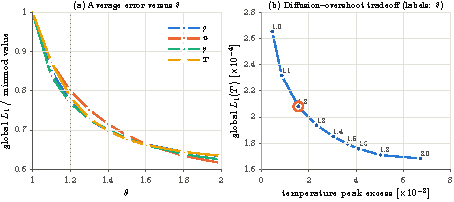
\includegraphics[width=\textwidth]{fig_theta_sweep.pdf}
\caption{(a) Average error relative to minmod as $\theta$ changes.  (b) Error
versus overshoot; each dot is one $\theta$, and the circle marks $\theta = 1.2$.}
\label{fig:theta}
\end{figure}

% ===========================================================================
\section{Key takeaways}
% ===========================================================================

\begin{enumerate}
  \item The solver tracks five particle groups that move through cells and relax
        toward a balanced state.  Their sums give density, velocity, temperature
        and pressure.
  \item The five-speed model reproduces the Euler equations exactly when $\tau$ is
        small.  $\tau$ adds a tiny amount of smoothing, mostly visible at the
        contact.
  \item MUSCL with the generalized-minmod limiter makes jumps sharp without adding
        wiggles.  SSP-RK3 steps forward in time accurately.
  \item The errors shrink at the rates expected for a problem with a shock and a
        contact.  All runs were stable and conserved mass and energy.
  \item The velocity ``stall'' at fine grids is a measurement quirk (shock position
        inside a cell), not a physics problem.
  \item $\theta = 1.2$ is a reasonable balance between smearing and overshoot.
\end{enumerate}

\paragraph{Good next steps.}
\begin{itemize}
  \item Halve the time step once on the finest grid to confirm time error is small.
  \item Test on a smooth problem (for example a small sound pulse) to confirm true
        second-order accuracy, which Sod cannot show.
  \item Run a $\tau$ study at a fixed time step to test the contact-width
        prediction directly.
  \item Before moving to 2D, pick a velocity set whose slow speed is larger than the
        flow speeds you expect.
\end{itemize}

\paragraph{More detail.}  Full derivations, proofs and extra tables are in the
companion technical report, \emph{Mathematical and Physical Foundations of the
KT-D1V5 Finite-Volume Discrete Boltzmann Solver} (\texttt{d1v5\_solver\_mathematics.pdf}).

% ===========================================================================
\section*{Glossary}
% ===========================================================================
\begin{description}[leftmargin=0pt,itemsep=2pt]
  \item[BGK collision] A simple rule that pulls the particle groups toward
        equilibrium at a rate set by $\tau$.
  \item[CFL number] How far the fastest particles move in one time step, measured in
        cells.
  \item[Contact] The boundary between two gases at the same pressure and speed but
        different density and temperature.
  \item[Equilibrium ($\feq$)] The balanced amounts of each particle group for a
        given density, velocity and temperature.
  \item[Finite volume] Dividing the tube into cells and tracking what flows through
        each cell's walls.
  \item[Limiter] A rule that caps the slope inside each cell to prevent fake
        wiggles.
  \item[MUSCL] Using a sloped line in each cell, instead of a flat value, to get
        sharper results.
  \item[Rarefaction] A smooth expansion where the gas thins out.
  \item[Relaxation time ($\tau$)] Roughly the time between collisions; smaller means
        closer to a frictionless gas.
  \item[Shock] A thin, sudden jump in pressure, density, velocity and temperature.
  \item[SSP-RK3] A three-stage time-stepping method that is accurate and does not
        create wiggles.
  \item[Upwinding] Taking information from the direction the particles are coming
        from.
\end{description}

% ===========================================================================
\begin{thebibliography}{99}
\small
\bibitem{BGK1954}
P.~L. Bhatnagar, E.~P. Gross, and M.~Krook, ``A model for collision processes in
gases. I,'' \emph{Physical Review} \textbf{94}, 511--525 (1954).
\href{https://doi.org/10.1103/PhysRev.94.511}{doi:10.1103/PhysRev.94.511}

\bibitem{ChapmanCowling1970}
S.~Chapman and T.~G. Cowling, \emph{The Mathematical Theory of Non-uniform Gases},
3rd ed., Cambridge University Press (1970).

\bibitem{Harten1983}
A.~Harten, ``High resolution schemes for hyperbolic conservation laws,''
\emph{Journal of Computational Physics} \textbf{49}, 357--393 (1983).
\href{https://doi.org/10.1016/0021-9991(83)90136-5}{doi:10.1016/0021-9991(83)90136-5}

\bibitem{KataokaTsutahara2004Euler}
T.~Kataoka and M.~Tsutahara, ``Lattice Boltzmann method for the compressible Euler
equations,'' \emph{Physical Review E} \textbf{69}, 056702 (2004).
\href{https://doi.org/10.1103/PhysRevE.69.056702}{doi:10.1103/PhysRevE.69.056702}

\bibitem{KurganovTadmor2000}
A.~Kurganov and E.~Tadmor, ``New high-resolution central schemes for nonlinear
conservation laws and convection--diffusion equations,'' \emph{Journal of
Computational Physics} \textbf{160}, 241--282 (2000).
\href{https://doi.org/10.1006/jcph.2000.6459}{doi:10.1006/jcph.2000.6459}

\bibitem{LeVeque2002}
R.~J. LeVeque, \emph{Finite Volume Methods for Hyperbolic Problems}, Cambridge
University Press (2002).
\href{https://doi.org/10.1017/CBO9780511791253}{doi:10.1017/CBO9780511791253}

\bibitem{ShuOsher1988}
C.-W. Shu and S.~Osher, ``Efficient implementation of essentially non-oscillatory
shock-capturing schemes,'' \emph{Journal of Computational Physics} \textbf{77},
439--471 (1988).
\href{https://doi.org/10.1016/0021-9991(88)90177-5}{doi:10.1016/0021-9991(88)90177-5}

\bibitem{Sod1978}
G.~A. Sod, ``A survey of several finite difference methods for systems of nonlinear
hyperbolic conservation laws,'' \emph{Journal of Computational Physics}
\textbf{27}, 1--31 (1978).
\href{https://doi.org/10.1016/0021-9991(78)90023-2}{doi:10.1016/0021-9991(78)90023-2}

\bibitem{Sweby1984}
P.~K. Sweby, ``High resolution schemes using flux limiters for hyperbolic
conservation laws,'' \emph{SIAM Journal on Numerical Analysis} \textbf{21},
995--1011 (1984).
\href{https://doi.org/10.1137/0721062}{doi:10.1137/0721062}

\bibitem{Toro2009}
E.~F. Toro, \emph{Riemann Solvers and Numerical Methods for Fluid Dynamics}, 3rd
ed., Springer (2009).
\href{https://doi.org/10.1007/b79761}{doi:10.1007/b79761}

\bibitem{vanLeer1979}
B.~van Leer, ``Towards the ultimate conservative difference scheme. V. A
second-order sequel to Godunov's method,'' \emph{Journal of Computational Physics}
\textbf{32}, 101--136 (1979).
\href{https://doi.org/10.1016/0021-9991(79)90145-1}{doi:10.1016/0021-9991(79)90145-1}
\end{thebibliography}

\end{document}
